We consider a modified version of the model used by \cite{DBLP:conf/sigecom/GaitondeT20,DBLP:journals/jacm/GaitondeT23}. There is a system of $n$ queues and $m$ servers. We divide time into discrete time steps $t=0,1, \dots$. In every step $t$, the following occurs. See the illustration in Figure \ref{fig:model}.
\begin{enumerate}
    \item Packets arrive at each queue $i$ according to a fixed probability $\lambda_i$. Formally, we model this by defining $B^i_t \sim \text{Bern}(\lambda_i)$ as an independent random variable that indicates whether a packet arrives at queue $i$ at time $t$. After arrival, each queue that contains at least one packet selects a server to which it attempts to send a single packet.

    \item Each server $j$ processes incoming packets as follows:
    (i) If the server's buffer is full, all received packets are rejected and returned to their respective queues. (ii) Otherwise, the server accepts one of the received packets, chosen uniformly at random, and places it in its buffer, rejecting the remaining packets. 
    (iii) The server then attempts to process the packet in its buffer. With probability $\mu_j$, the processing succeeds, and the packet is removed from the buffer. If the processing fails, the packet remains in the buffer.
        
    \item Any packets not accepted into a server's buffer are returned to their respective queues. Each queue receives bandit feedback based on the outcome of sending its packet: a reward of zero if the packet was not accepted by the server a reward of one if the packet was successfully placed in the server's buffer.\footnote{Feedback 
    % for packets placed in buffers 
    is received immediately after a packet is placed in the buffer, not necessarily when it is successfully processed.}
    
\end{enumerate}

\begin{figure}[t!]
\centering
\resizebox{0.36\textwidth}{!}{%
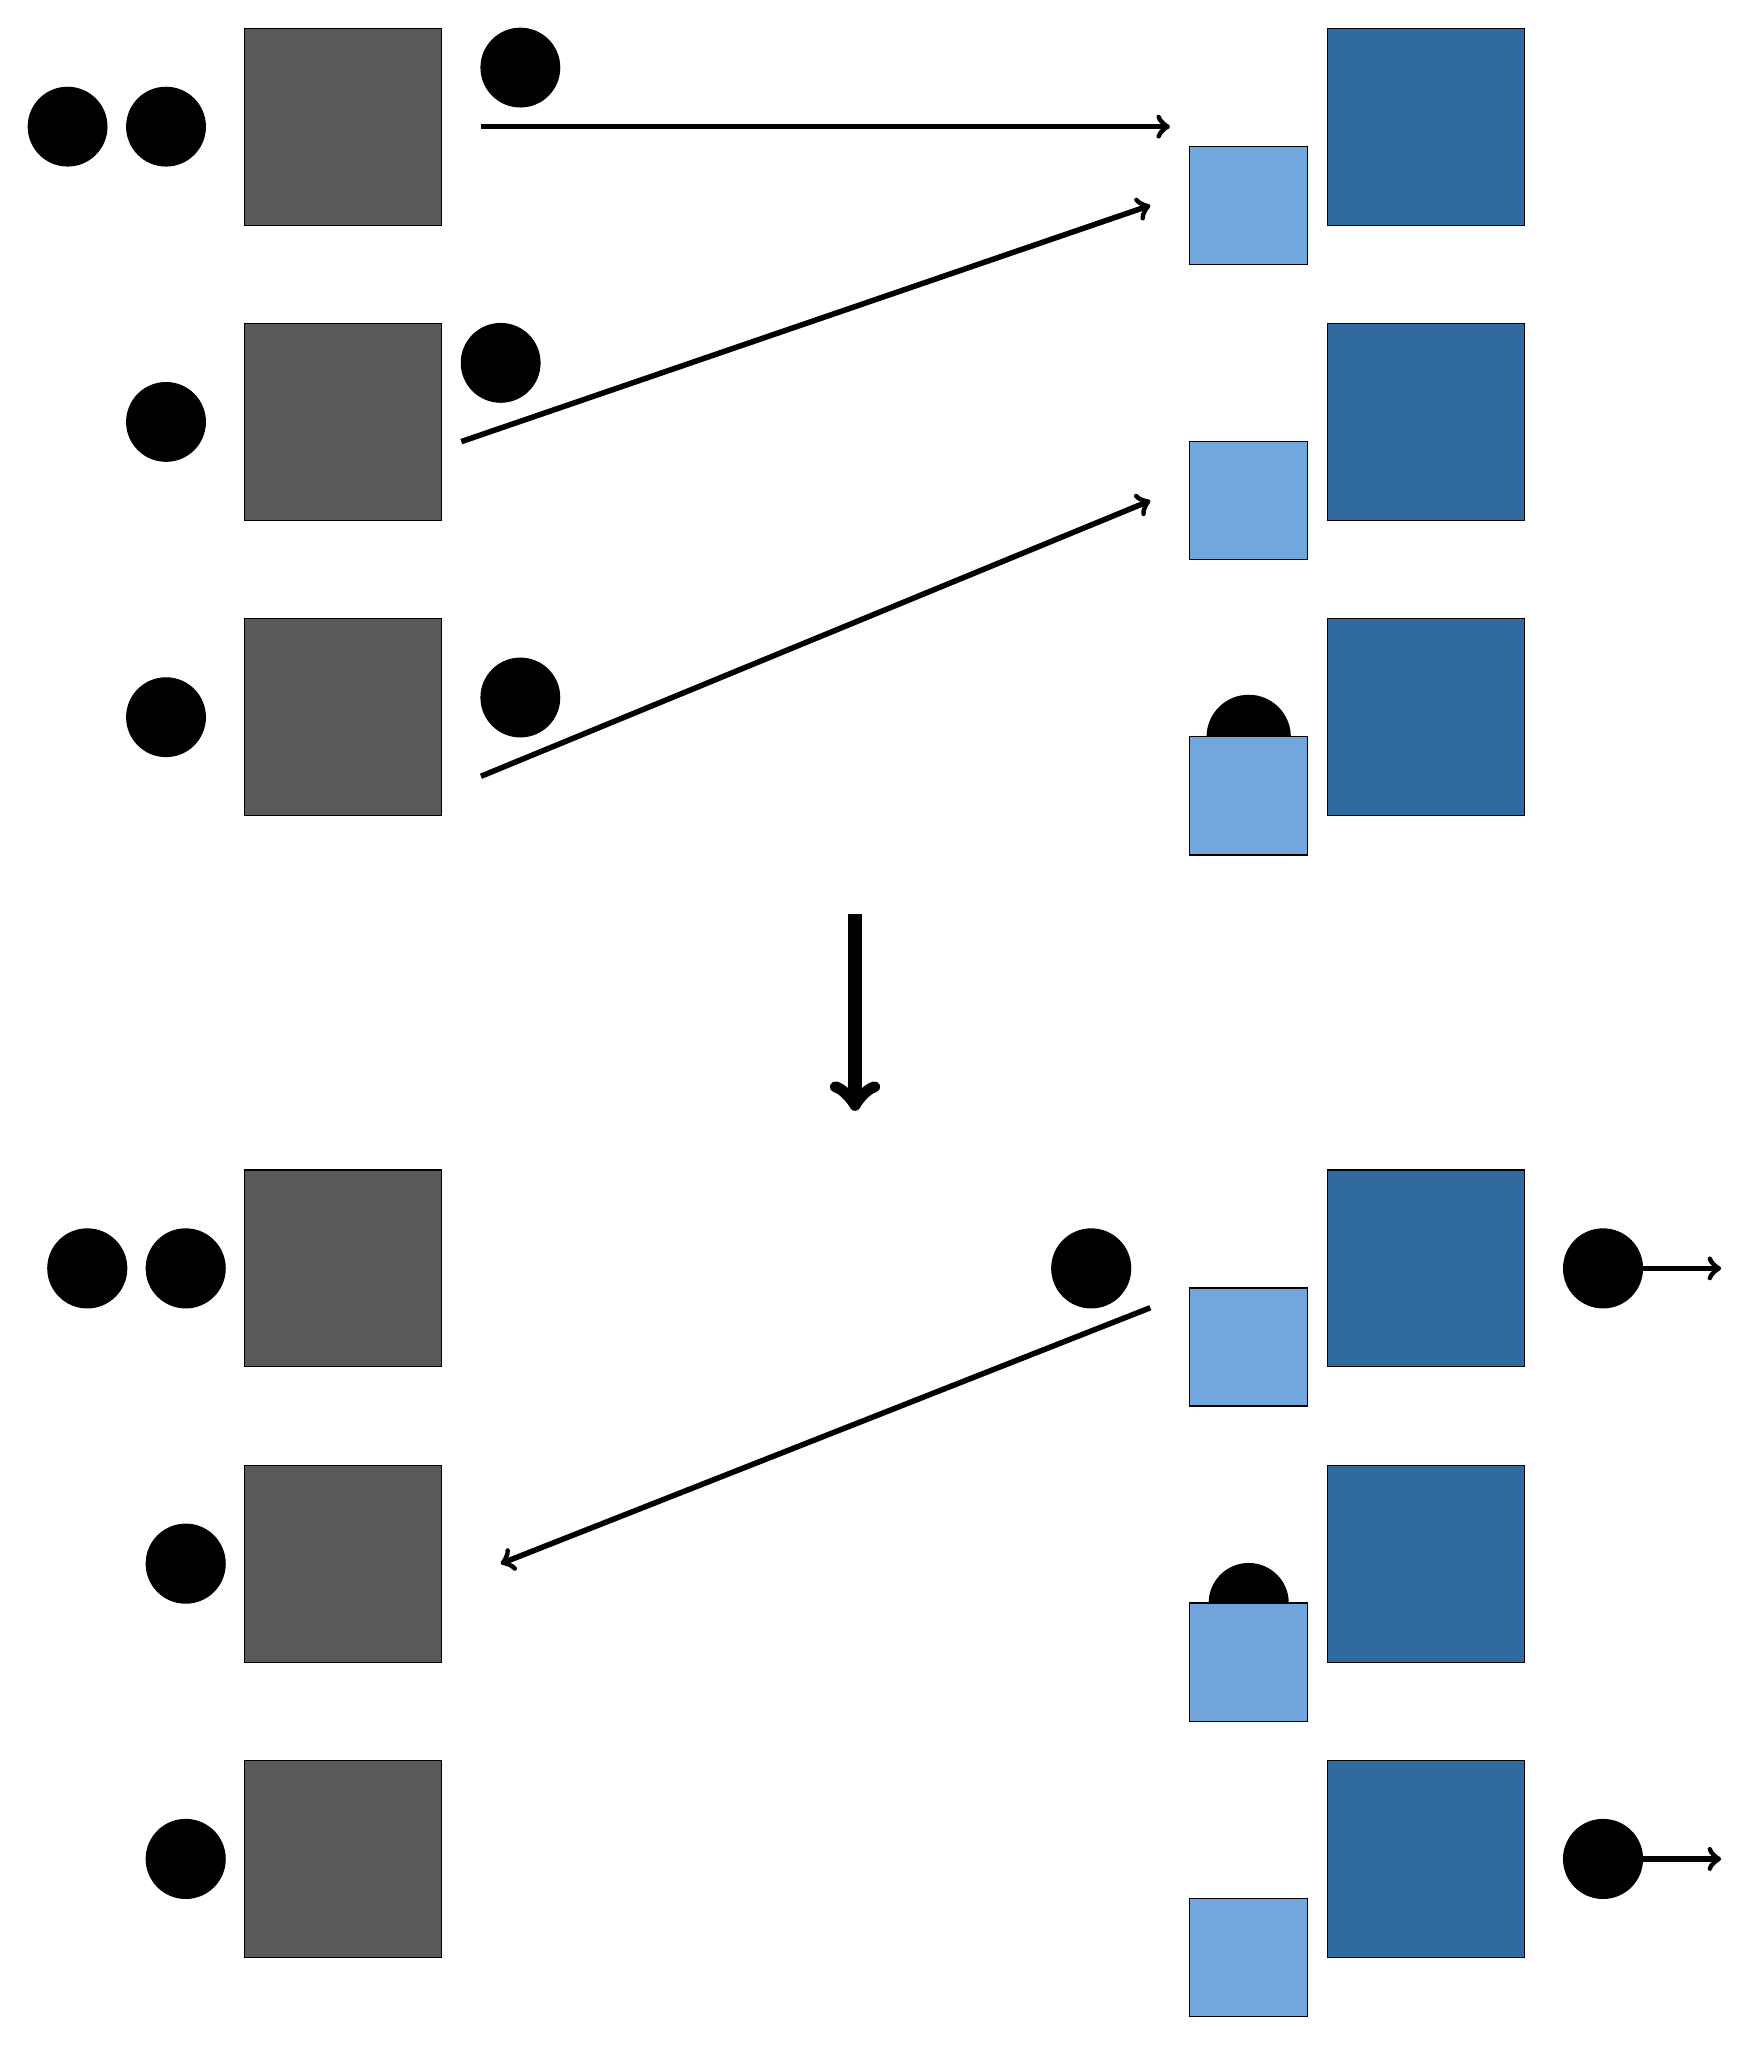
\begin{tikzpicture}
\tikzstyle{every node}=[font=\LARGE]
\draw [ fill={rgb,255:red,49; green,106; blue,158} ] (12.5,9.75) rectangle  node {\LARGE 
} (15,7.25);
\draw [ fill={rgb,255:red,49; green,106; blue,158} ] (12.5,6) rectangle (15,3.5);
\draw [ fill={rgb,255:red,49; green,106; blue,158} ] (12.5,2.25) rectangle (15,-0.25);
\draw [ fill={rgb,255:red,89; green,89; blue,89} ] (-1.25,9.75) rectangle (1.25,7.25);
\draw [ fill={rgb,255:red,89; green,89; blue,89} ] (-1.25,6) rectangle (1.25,3.5);
\draw [ fill={rgb,255:red,89; green,89; blue,89} ] (-1.25,2.25) rectangle (1.25,-0.25);
\draw [line width=2pt, ->] (1.75,8.5) .. controls (6,8.5) and (6.25,8.5) .. (10.5,8.5) ;
\draw [line width=2pt, ->] (1.5,4.5) -- (10.25,7.5);
\draw [line width=2pt, ->] (1.75,0.25) -- (10.25,3.75);

\draw [ fill={rgb,255:red,0; green,0; blue,0} ] (2.25,9.25) circle (0.5cm);
\draw [ fill={rgb,255:red,0; green,0; blue,0} ] (2,5.5) circle (0.5cm);
\draw [ fill={rgb,255:red,0; green,0; blue,0} ] (2.25,1.25) circle (0.5cm);
\draw [ fill={rgb,255:red,0; green,0; blue,0} ] (-2.25,8.5) circle (0.5cm);
\draw [ fill={rgb,255:red,0; green,0; blue,0} ] (-2.25,4.75) circle (0.5cm);
\draw [ fill={rgb,255:red,0; green,0; blue,0} ] (-2.25,1) circle (0.5cm);
\draw [ fill={rgb,255:red,0; green,0; blue,0} ] (-3.5,8.5) circle (0.5cm);
\draw [line width=5pt, ->] (6.5,-1.5) -- (6.5,-4);
\node [font=\LARGE] at (0.5,8) {};
\node [font=\LARGE] at (0.5,8) {};
\draw [ fill={rgb,255:red,89; green,89; blue,89} ] (-1.25,-4.75) rectangle (1.25,-7.25);
\draw [ fill={rgb,255:red,89; green,89; blue,89} ] (-1.25,-8.5) rectangle (1.25,-11);
\draw [ fill={rgb,255:red,89; green,89; blue,89} ] (-1.25,-12.25) rectangle (1.25,-14.75);
\draw [ fill={rgb,255:red,49; green,106; blue,158} ] (12.5,-4.75) rectangle (15,-7.25);
\draw [ fill={rgb,255:red,49; green,106; blue,158} ] (12.5,-8.5) rectangle (15,-11);
\draw [ fill={rgb,255:red,49; green,106; blue,158} ] (12.5,-12.25) rectangle (15,-14.75);
\draw [ fill={rgb,255:red,112; green,168; blue,219} ] (10.75,8.25) rectangle (12.25,6.75);
\draw [ fill={rgb,255:red,112; green,168; blue,219} ] (12.25,3) rectangle (10.75,4.5);
\draw [line width=2pt, ->] (10.25,-6.5) -- (2,-9.75);
\draw [ fill={rgb,255:red,0; green,0; blue,0} , line width=2pt ] (11.5,0.75) circle (0.5cm);
\draw [ fill={rgb,255:red,113; green,167; blue,220} ] (10.75,0.75) rectangle (12.25,-0.75);
\draw [ fill={rgb,255:red,113; green,167; blue,220} , line width=0.5pt ] (10.75,-6.25) rectangle (12.25,-7.75);
\draw [ fill={rgb,255:red,113; green,167; blue,220} , line width=0.5pt ] (10.75,-14) rectangle (12.25,-15.5);
\draw [ fill={rgb,255:red,0; green,0; blue,0} , line width=0.5pt ] (11.5,-10.25) circle (0.5cm);
\draw [ fill={rgb,255:red,0; green,0; blue,0} , line width=0.5pt ] (16,-13.5) circle (0.5cm);
\draw [ fill={rgb,255:red,0; green,0; blue,0} , line width=0.5pt ] (16,-6) circle (0.5cm);
\draw [ fill={rgb,255:red,0; green,0; blue,0} , line width=0.5pt ] (9.5,-6) circle (0.5cm);
\draw [ fill={rgb,255:red,0; green,0; blue,0} , line width=0.5pt ] (-2,-6) circle (0.5cm);
\draw [ fill={rgb,255:red,0; green,0; blue,0} , line width=0.5pt ] (-2,-9.75) circle (0.5cm);
\draw [ fill={rgb,255:red,0; green,0; blue,0} , line width=0.5pt ] (-2,-13.5) circle (0.5cm);
\draw [ fill={rgb,255:red,0; green,0; blue,0} , line width=0.5pt ] (-3.25,-6) circle (0.5cm);
\draw [line width=2pt, ->] (16.25,-6) -- (17.5,-6);
\draw [line width=2pt, ->] (16,-13.5) -- (17.5,-13.5);
\draw [ fill={rgb,255:red,113; green,166; blue,221} ] (10.75,-10.25) rectangle (12.25,-11.75);
\end{tikzpicture}
}%
\caption{A three-queue, three-server system in a single time step. Discs represent packets; left squares are queues, right squares are servers, and small squares are buffers. In this time step, two packets are sent to the top server, one of them is accepted into a buffer and then processed, the other one is returned to its queue. For the other two servers, one admits a packet into a buffer but fails to serve it and one processes a packet that was in its buffer.}
\label{fig:model}
\end{figure}

\begin{definition}
    We say that a system with a schedule for sending packets is \emph{stable} if the expected number of packets waiting to be sent or served in the system is bounded by a constant at all times. We allow the constant to depend on the number of queues or servers and the parameters of the system, but it may not grow with time $T$. 
\end{definition}

It is clear that if $\sum_i \lambda_i >\sum_j \mu_j$ then even a fully coordinated system cannot be stable, and the total number of packets waiting at the queues must grow linearly in time. In the case of a single queue with a single server, $\lambda <\mu$ is the necessary and sufficient condition for keeping the packets remaining in the system bounded by a constant (which depends on the gap in the inequality) at all times. The analogous condition is clearly necessary but not sufficient in case of multiple servers. 
\begin{lemma}
    Consider an example with 1 queue and 2 servers, each with $\mu=\frac12$. We claim that $\lambda < \frac{23}{24}<1$ is needed for the system to be stable even with full coordination.
\end{lemma}
\begin{proof}
    To see why this is true, consider 3 consecutive time steps. To analyze the maximum processing rate we look at the scenario where the queue sends a packet in each of these steps. We claim that with probability $1/8$ it holds that in one of the three times the queue must fail to have a packet accepted by a server. To see this, assume the following.
    \begin{itemize}
        \item Assume that at step 1 the queue sends a packet to one of the servers, which fails to serve it, but may keep it in its buffer. This event has probability at least $\frac12$. 
        \item With full coordination, the queue is aware of the first buffer being full and can try to send the next packet to the second server. Assume that at this step neither of the two servers succeed in sending packets, but as before, may accept the new packet into its buffer. This event has probability at least $\frac14$.
        \item Even if the first two packets were accepted into buffers, in this case, at the third time step, both buffers are full, and so there is no place for the queue to send.
    \end{itemize}
This proves that during a set of consecutive three steps the maximum expected service rate is at most $$\frac{\frac18\cdot 2+\frac78 \cdot 3}{3}=\frac{23}{24}.$$
Thus, if the arrival rate $\lambda$ is higher, we will have a buildup of the queue linear in $T$.  
\end{proof}